\begin{figure*}[b!]
    \centering
    \begin{minipage}{0.69\textwidth}
        \resizebox{\textwidth}{!}{
            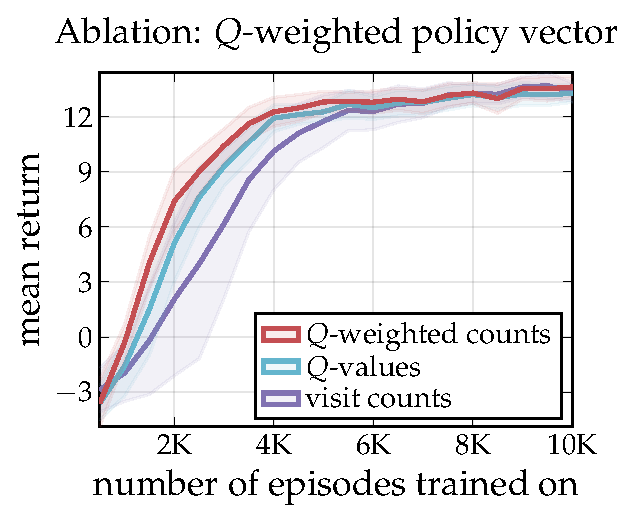
\includegraphics{figures/ablations/plot_ablation_q_weighting.pdf}
            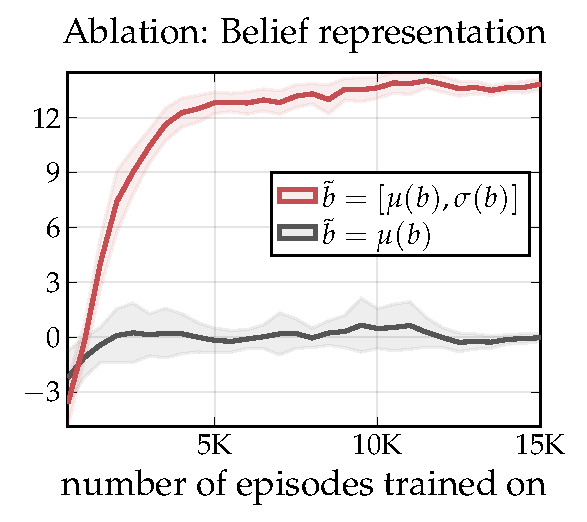
\includegraphics{figures/ablations/plot_ablation_belief_rep.pdf}
            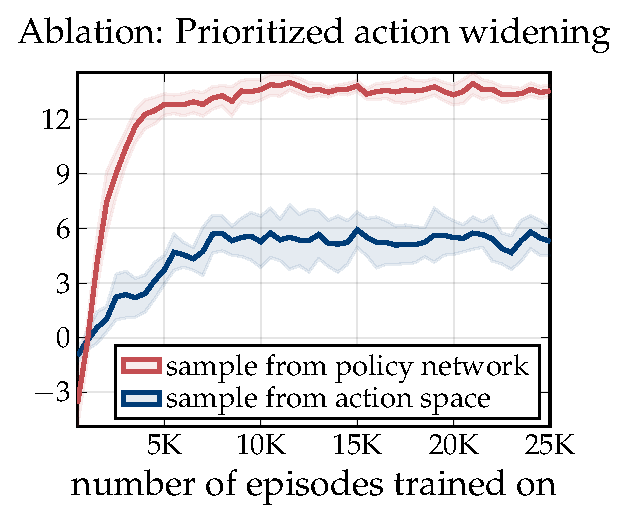
\includegraphics{figures/ablations/plot_ablation_action_selection.pdf}
    }
    \end{minipage}%
    \hspace*{3mm}
    \begin{minipage}{0.3\textwidth}
        \resizebox{\textwidth}{!}{%
            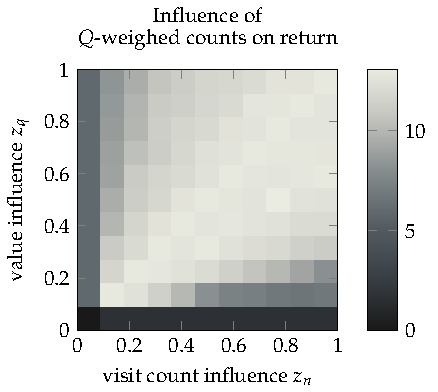
\includegraphics{figures/results/z_sweep.pdf}
        }
    \end{minipage}

    \begin{minipage}[t]{0.69\textwidth}
        \caption{
        Ablation study in \textsc{LightDark}$(10)$.
        (Left) Learning is faster when policy network is trained using $Q$-weighted visit counts.
        (Middle) Incorporating belief uncertainty is crucial for learning.
        (Right) Action widening from the policy network shows significant improvement.
        The same red curves are shown and one std is shaded from three seeds with exponential smoothing with weight $0.6$.}
        \label{fig:ablations}
    \end{minipage}%
    \hspace*{3mm}
    \begin{minipage}[t]{0.3\textwidth}
        \caption{Ablation study in \textsc{RockSample}$(20,20)$.
        Combining value and count information leads to the highest return. The diagonal is identical due to the $\argmax$ of \cref{eq:policy_q_weight}.}
        \label{fig:z_sweep}
    \end{minipage}
\end{figure*}
